
%(BEGIN_QUESTION)
% Copyright 2012, Tony R. Kuphaldt, released under the Creative Commons Attribution License (v 1.0)
% This means you may do almost anything with this work of mine, so long as you give me proper credit

%Suppose a technician wishes to use a loop calibrator to simulate a 4-20 mA signal to a controller, and decides to connect the loop calibrator to the circuit like this:
Anta at en automatiker ønsker å bruke en loop-kalibrator til å simulere et 4-20mA til en regulator. Han kobler den opp slik som tegningen viser. 

$$\includegraphics[width=15.5cm]{i00011x01.eps}$$

%Explain why this is an improper use of the loop calibrator, and what will happen if the technician tries to simulate a 9 mA signal this way.  Finally, identify the proper way to use the loop calibrator to simulate a transmitter signal.
Forklar hvorfor denne måten og koble på ikke vil fungere, og hva som vil skje om han prøver å simulere 9 mA på denne måten? Forklar hvordan en loop-kalibrator skal kobles for å simulere transmitter signalet. 

\vfil

\underbar{file i00011no}
\eject
%(END_QUESTION)





%(BEGIN_ANSWER)

This is a graded question -- no answers or hints given!

%(END_ANSWER)





%(BEGIN_NOTES)

The problem here is that the transmitter is still in the circuit, passing its own current.  The 9 mA passed by the loop calibrator in ``simulate'' mode will become {\it added} to the transmitter's current to form a larger total current seen at the 250 ohm resistor.

The proper way to use the loop calibrator is like this:

$$\includegraphics[width=15.5cm]{i00011x02.eps}$$

%INDEX% Electronics review: 4-20 mA loop calibrator (test equipment)

%(END_NOTES)


